\label{sec:proj}
The core of our project is the calculation of semi-leptonic decays of the $D_s$ mesons.
The raw data produced with the HPC facilities
contributes to the determination of 
the total inclusive decay rate for the process $D_s \to X\ell\nu$ and with the same 
data the decay constants $f_{D_s}$ and $f_D$ can be computed.

The computation proposed here will be using the Wilson-clover twisted
mass regularisation of lattice QCD~\cite{Alexandrou:2018egz}. The up/down quarks will be treated
in a fully unitary setting. In order to avoid flavour mixing lattice artifacts 
in the unitary strange/charm sector of this regularisation, we use a
mixed action approach for strange and charm quarks: so-called
Osterwalder-Seiler type~\cite{Frezzotti:2004wz} strange and charm quark doublets
$(s^+ , s^-)^T$ and $(c^+ , c^- )^T$ are added with bare
twisted strange and charm quark mass $\pm \mu_s$ and $\pm \mu_c$
tuned to reproduce the physical mass of the $\phi$ and $J/\Psi$
mesons, respectively, as described in Appendix C of
Ref.\cite{ExtendedTwistedMass:2022jpw}. For more details, we refer to
this reference.

Before discussing the two sub-projects we would like to point out that a
successful implementation of the proposed project will produce not
only phenomenologically interesting results, but it will also be the
basis for a future extension towards B mesons using the ideas we have
put forward in Ref.~\cite{ETM:2009sed}.

\subsection{Sub-project 1: total inclusive decay rate $D_s \to X\ell\nu$}

By using the optical theorem, the total inclusive decay rate for the
process $D_s \to X\ell\nu$ can be written as
\begin{equation} 
  \Gamma = G^2_F\left\{ |V_{cd} |^2 \Gamma_{cd} + |V_{cs} |^2 \Gamma_{cs} + |V_{us} |^2 \Gamma_{su}
  \right\}\,,
\end{equation}
where the different contributions on the right side correspond at the quark level to the weak
transitions $c \to d$, $c \to s$ and $s \to u$ respectively. Each contribution can be written as
\begin{equation}\label{eq:Gamma_fg}
  \Gamma_{fg}=\int \frac{d^3p_\nu}{(2\pi)^32E_\nu}\frac{d^3p_\ell}{(2\pi)^32E_\ell}
  L_{\mu\nu}(p_\ell, p_\nu) H^{\mu\nu}_{fg}(p,p-p_\ell-p_\nu)\,,
\end{equation}
where the leptonic tensor is given by
\begin{equation}
  L_{\mu\nu}(p_\ell, p_\nu) =4\left\{p_\ell^\mu p_\nu^\nu +p_\ell^\nu
  p_\nu^\mu - g^{\mu\nu} p_\ell\cdot p_\nu+
  i\epsilon_{\mu\nu\alpha\beta} p_\ell^\alpha p_\nu^\beta\right\}\,, 
\end{equation}
while the hadronic tensor reads
\begin{equation}
  H^{\mu\nu}_{fg}(p,p_X)=\frac{1}{2m_{D_s}}\langle D_s| J^\mu_{fg}(0)(2\pi)^4
  \delta^4(\mathbb{P}-p_x) J^{\nu\dagger}_{gf} (0)| D_s\rangle\,.
\end{equation}
$\mathbb{P}$ is the QCD four momentum operator and $J_{gf}$ are the
relevant Minkowski weak currents $J_{gf}^\mu(x)=i\bar
g(x)\gamma^\mu(1-\gamma_5)f(x)$. 
In this project we will focus on the calculation of $\Gamma_{cd}$ and $\Gamma_{cs}$ while we will neglect the contribution of $\Gamma_{su}$ which is suppressed by the integration over the phase space of \eqref{eq:Gamma_fg}.
The calculation of $\Gamma_{cs}$ requires computing disconnected diagrams which is computationally more challenging than the connected part.
% since they need the all to all propagator.
%While many methods are being used and developed,
%like deflation with hierarchical probing for disconnected diagrams 
%\cite{Stathopoulos:2013aci, Gambhir:2016jul} 
%(See also a summary of the  methodology applied for these calculations in Sec. 10.1.1. of \cite{FlavourLatticeAveragingGroupFLAG:2021npn}),
%they remain a numerically more expensive than the connected diagrams.
On the other hand the contribution coming from disconnected diagrams is expected to be small due to OZI-suppression rule.
For this reason we will carry out the computation of the disconnected diagram in a separate project focusing here only on the computation of $\Gamma_{cd}$ and the connected part of $\Gamma_{cs}$.

From now on we will drop the indices $fg$ and the procedure we are describing will be equivalent for the $cd$ and $cs$ contribution,
moreover in the rest frame of the $D_s$ meson we have $p=(m_{D_s},\bm{0})$ thus we simplify the notation of 
$H^{\mu\nu}(p_X)\equiv H^{\mu\nu}_{fg}(p,p_X)$.
The hadronic tensor $H_{\mu\nu}$ is
the spectral density of the quantity  
\begin{equation}
  M_{\mu\nu}(t,{\bf q})= \int_0^{\infty}d \omega H_{\mu\nu} (\omega,{\bf q}) e^{-\omega t}\,,\quad \text{with}\quad p_X=(\omega,\bm{q})\,.
\end{equation}
$H_{\mu\nu}$ can be reconstructed from $M$ using the method presented in
Ref.~\cite{Hansen:2019idp}. $M$ can be directly computed from the
ratio of Euclidean lattice correlators
\begin{gather}
  M_{\mu\nu}(t_2-t_1,{\bf q})=\frac{C_{\mu\nu}(t_{snk},t_2,t_1,t_{src};q)}{e^{-(t_{snk}-t_2)}  C(t_1-t_{src}) }\label{eq:ratio_4pt_2pt}\\
  \label{eq:4pt}
  C_{\mu\nu}(t_{snk},t_2,t_1,t_{src};q)=\int d^3x e^{i{\bf q}\cdot {\bf x}}
  \langle D_s({\bf 0}, t_{snk}) J^{\dagger}_\mu({\bf x},t_2)  J_\nu(0,t_1)
  D_s^\dagger({\bf 0}, t_{src})\rangle\,,\\
  \label{eq:2pt}
  C(t_{snk}-t_{src}) =  \langle D_s({\bf 0}, t_{snk})
  D_s^\dagger({\bf 0}, t_{src})\rangle\,.
\end{gather}
In general, the inverse problem represented by the extraction of
hadronic spectral densities from Euclidean correlators is notoriously
ill-posed. Recently, a method to cope with these problems has been
proposed in Ref.~\cite{Hansen:2019idp}. It consists of treating the
integrals mentioned above with some $C_\infty$ kernel $K_\sigma$  
\begin{equation}
  H^\sigma_{\mu\nu}(\omega^*, {\bf q})= \int d \omega K_\sigma( \omega^*,\omega ) H_{\mu\nu}(\omega, {\bf q})\,,
\end{equation}
making the inverse problem well posed and $H^\sigma_{\mu\nu}$ computable.
In our case the phase space integration in \eqref{eq:Gamma_fg}
provides a sharp smearing kernel function $\theta$. Following
Refs.~\cite{Gambino:2020crt, Gambino:2022dvu}, the phase space integral over
\eqref{eq:Gamma_fg} can be written as 
\begin{gather}
  \frac{48 \pi^4}{m_{D_s}^5}\frac{d\Gamma}{d \bm{ \omega^2} }
  =\sum_{l=0}^2 |\bm{\omega}|^{3-l}\int_0^{\infty}d \omega_0 \theta(\omega_0^{max}-\omega_0) Z^l\,,\quad\quad {\omega}_0^{max}=1-|\bm{\omega}|\,,\\
  Z^2=Y_3-2Y_1\,,\quad Z^1=2(Y_3-2Y_1-Y_4)\,,\quad Z^0=Y_2+Y_3-2Y_4\,.
\end{gather}
Moreover, the $Y_i$ can be directly computed from the Euclidean
hadronic tensor $H^{\mu\nu}$ as follows 
\begin{align}
  &Y^1=-m_{D_s}\sum_{ij}\hat{n}^i\hat{n}^j H^{ij}(p,q)\,,&& Y^2=-m_{D_s}H^{00}(p,q)\,,\\
  &Y^3=m_{D_s}\sum_{ij}\hat{\omega}^i\hat{\omega}^j H^{ij}(p,q)\,,&&
  Y^4=-im_{D_s}\sum_{i}\hat{\omega}^i H^{0i}(p,q)\,,&
\end{align} 
with $\hat{n}$ a unit vector orthogonal to $\bm\omega$.
Thus the phase space integral provides us a $\theta$-function smearing
kernel. However, the $\theta$-function is not smooth, which is why we
will use a $C_\infty$ kernel that 
after taking the infinite volume limit, the 
$\theta$-function is recovered as $\sigma\to0$, i.e. $\lim_{\sigma\to 0} K_\sigma(x^*,x)=\theta(x^*-x)$.
%such that the step-function is recovered in the limit $\sigma\to0$, i.e.
%$\lim_{\sigma\to 0} \theta_\sigma(x)=\theta(x)$.
 Therefore,
\begin{gather}
  \frac{48 \pi^4}{m_{D_s}^5}\frac{d\Gamma}{d \bm{ \omega^2} }
  =\lim_{\sigma\to 0}\sum_{l=0}^2 |\bm{\omega}|^{3-l}\int_0^{\infty}d \omega_0 K_\sigma(\omega_0^{max},\omega_0) Z^l\,.
\end{gather}
The spectral reconstruction can be performed at the analysis stage. Thus,
the main cost of this calculation is the production of the
four-point function \eqref{eq:4pt}. In the case of the $c\to d$ weak
transition the corresponding required Wick contractions are shown in
Fig.~\ref{fig:4pt}.

The renormalization constants necessary to renormalise the ratio of
correlators \eqref{eq:ratio_4pt_2pt} $Z_A$ and $Z_V$ are already
computed in previous work of ETMC~\cite{ExtendedTwistedMass:2022jpw}. 

\begin{figure}
  \centering
  \begin{tikzpicture}
    \begin{feynman}[scale=1.5]		 
      \vertex[anchor=east,blob, fill=black!0!] (a) at (0,0) {\(D_s^\dagger\)};
      \vertex[anchor=east,blob, fill=black!0!]  (J1) at (1,0.8) {\(J_W\)};
      \vertex[anchor=east,blob, fill=black!0!] (J2) at (2.4,0.8) {\(J_W\)};
      \vertex[anchor=west,blob, fill=black!0!] (b) at (3,0) {\(D_s\)};
      \vertex (s1) at (3.4,-0.4) ;
      \vertex (s2) at (3.4, 0.4) ;
      \vertex (s3) at (2.6, 0.7) ;
      \vertex (s4) at (1.8, 1) ;
      
      \diagram*{
        %				(a) --[fermion,  half right,looseness=0.5,edge label=$s$] (b);
	(b) --[fermion, red, out=220, in=320,edge label=$s$,swap] (a);
        
	(a) --[fermion, sand, edge label=$c$] (J1) ;
	(J1) --[fermion, blue, edge label=$d$, reversed momentum'=$\bf{q}$] (J2);
	(J2) --[fermion, sand ,edge label=$c$] (b);			
	(s1) --[->, half right, edge label=sequential,swap] (s2);
	(s3) --[->, half right, edge label=sequential,swap] (s4);
      };
    \end{feynman}
    \begin{feynman}[scale=1.5]		 
      \vertex[anchor=east,blob, fill=black!0!] (a) at (6.5,0) {\(D_s^\dagger\)};
      \vertex[anchor=west,blob, fill=black!0!] (b) at (9.5,0) {\(D_s\)};
      
      \diagram*{
	%				(a) --[fermion,  half right,looseness=0.5,edge label=$s$] (b);
	(b) --[fermion, red, out=220, in=320,edge label=$s$,swap] (a);
	(a) --[fermion, sand, out=40, in=140,edge label=$c$,swap] (b);
      };
    \end{feynman}	
  \end{tikzpicture}
  \caption{On the left: Wick contractions required for the calculation of the correlator \eqref{eq:4pt} for the contribution $cd$. For the contribution $cs$ the $d$-quark propagator must be replaced with and $s$-quark propagator. On the right: Wick contractions required for the calculation of the correlator \eqref{eq:2pt} .}
  \label{fig:4pt}
\end{figure}	

As mentioned already, we have performed a first exploratory
investigation of the differential decay rate on ensemble cB211.072.64
in order to understand the feasibility of the proposed calculation. We
used 300 gauge configurations with three stochastic sources each
(see below for how stochastic sources are used here)
and we compute only the $cd$ contribution. The
resulting differential decay rate is shown in Fig.~\ref{fig:Gamma_B64}
for four values of the square momentum of the final hadronic state. Apart from the statistical
accuracy, which appears satisfactory, we also wanted to understand how
to choose the time-separations appropriately. For one of the values of
the momenta we have performed the calculation for different choices
for the times $t_{snk}$, $t_2$ and the minimal value of $t_1$ included
in the spectral reconstruction. However, within errors, all three
choices give compatible results.

For the calculation proposed here we plan to stick to the most
conservative choice, namely $t_{snk}=56$, $t_2=40$ and $t_1=16$,
corresponding to the blue circles in Fig.~\ref{fig:Gamma_B64}.
For the ensembles at the other lattice spacings and volumes we plan to keep the
time separations constants in physical units. 


\begin{figure}
  \centering
  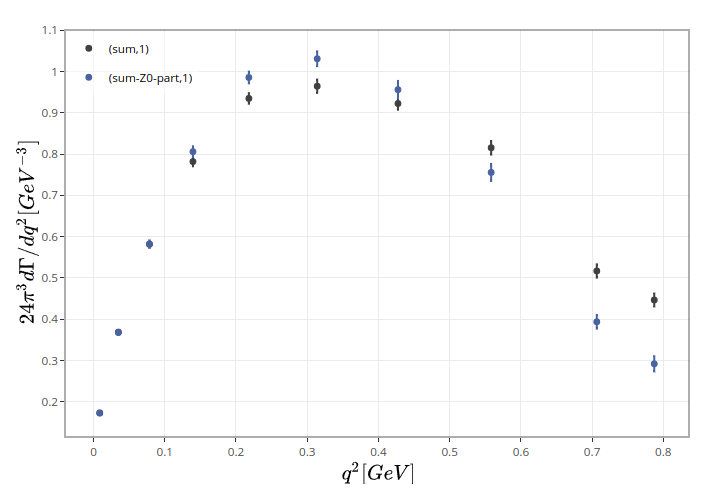
\includegraphics[scale=0.7]{plots/dgamma_dq2.png}
  \caption{Preliminary values of the differential decay rate of
    $D_s\to X\ell\nu$ (only the contribution coming from $\Gamma_{cd}$) as a function of the squared momentum for the
    extrapolated to the continuum limit..}
  \label{fig:dGammadq_Ds}
\end{figure}

\subsection{Sub-project 2: decay constant $f_D$ and $f_{D_s}$}

From the two-point function \eqref{eq:2pt} we can extract the decay
constant of the corresponding pseudo-scalar (PS) meson as 
\begin{equation}
  f_\mathrm{PS}=(\mu_f+\mu_{f'})\frac{\langle 0| P_{ff'}|
    \mathrm{PS}\rangle}{M_\mathrm{PS}^{ff'}\sinh(M_\mathrm{PS}^{ff'})}\, 
\end{equation}
where the matrix element is extracted from the correlation function
\eqref{eq:2pt} at large time separations. The PS-meson is made out of
valence quark flavours with bare masses $\mu_f$ and $\mu_{f'}$ , and
its mass is denoted by $M_\mathrm{PS}^{ff'}$. We plan to compute the
decay constant for the $D_s$ and $D$ meson, thus $f=c$ and $f'=s,d$. 

\endinput
